%%%%%%%%%%%%%%%%%%%%%%%%%%%%%%%%%%%%%%%%%%%%%%%%%%%%%%%%%%%%%%%%%%%%%%%%%%%%%%%%%%%%%%%%%%%
%%%% Die Dokumentenklasse und ihre Optionen %%%%%%%%%%%%%%%%%%%%%%%%%%%%%%%%%%%%%%%%%%%%%%%
\documentclass[captions=tableheading, 12pt, headings=small, parskip=half]{scrartcl}

%%%%%%%%%%%%%%%%%%%%%%%%%%%%%%%%%%%%%%%%%%%%%%%%%%%%%%%%%%%%%%%%%%%%%%%%%%%%%%%%%%%%%%%%%%%
%%%% LaTeX-Pakete %%%%%%%%%%%%%%%%%%%%%%%%%%%%%%%%%%%%%%%%%%%%%%%%%%%%%%%%%%%%%%%%%%%%%%%%%
\usepackage[utf8]{inputenc}
\usepackage[T1]{fontenc}
\usepackage[ngerman]{babel}
\usepackage{setspace,               % Zeilendurchschuss verändern (\doublespacing,\onehalfspacing)
            booktabs,               % Schöne Tabellen
            amsmath,                % Mathepackage der American Mathematical Society
            amsfonts,               % Paket für schönere mathematische Schriftarten
            amssymb,                % Paket für schönere mathematische Symbole
            bbm, 					% Blackboard-Style im Mathemodus
            bm, 					% Bold-Symbols im Mathemodus
            enumitem, 				% Anpassungen der enumerate-Umgebung
            graphicx,               % Paket zum Laden von Graphiken
            lmodern,                % Schrifttyp, der mit Microtype zusammenarbeitet
            nicefrac,				% Schräge Brüche
            csquotes,				% für Anführungszeichen
            microtype,              % Typographische Korrekturen bei Umbrüchen
            hyperref,				% url-Befehl
            calligra,
            setspace,
            multirow,
            float,
            eurosym,
            epstopdf,
            lscape,
            longtable,
            calc,
            dsfont
}
\usepackage[left=2.5cm,right=2.5cm,top=2cm,bottom=2cm]{geometry} % Seiteneinrichtung
%\usepackage{geometry} % Seiteneinrichtung

\usepackage{dcolumn}
\newcolumntype{d}[1]{D{.}{.}{#1}}


% \graphicspath{{C:\Users\stapperm\Documents\Econometrics 1\Code}}

\newcounter{tfno}
\newcommand{\mybox}{\resizebox{.5cm}{!}{\raisebox{-.5ex}{$\Box$}}}
%
\setcounter{tfno}{0} %% moved here
\newenvironment{truefalse}{%
	%\setcounter{tfno}{0}  %% moved up
	\renewcommand\arraystretch{1.5}
	\setlength\LTleft{0pt}
	\setlength\LTright{0pt}
	\begin{longtable}{>{\stepcounter{tfno}\thetfno.}cp{.5\textwidth}@{\extracolsep{\fill}}cc}
		\multicolumn{1}{r}{}&  & \fbox{\parbox{\widthof{True}}{True}} & \fbox{\parbox{\widthof{False}}{False}}  \\
	}{%
	\end{longtable}
	\renewcommand\arraystretch{1}
}
\newcommand\tfquestion[1]{ & #1 & \mybox  & \mybox  \\}


\begin{document}

\begin{table}[H]
	\begin{tabular}{lr}
		& \multirow{4}{*}{
\includegraphics[width = 8cm]{Code2/wwu_logo.png}}\\
		Dr. Willi Mutschler& \\
		M.Sc. Manuel Stapper & \\
		Summer term 2018 \hphantom{MMMMMMMMMMM}& 
	\end{tabular}
\end{table}
\vspace{1cm}
\begin{center}
	{\Large Econometrics II} \\
	-- Exercise Book --
\end{center}

\section*{\underline{Exercise 1}}
It is assumed that the connection between consumption $c_t$ and income $y_t$ is linear:
\[c_t = \alpha + \beta y_t + u_t\]
For a study the following data is collected:
 \begin{table}[h!]
 	\centering
 	\begin{tabular}{cd{5.0}d{3.0}d{3.0}d{3.0}d{3.0}d{3.0}d{3.0}d{3.0}d{3.0}d{3.0}d{3.0}d{3.0}d{3.0}}
 		\toprule
 		\toprule
 		\boldsymbol{$t$} & 1 & 2 & 3 & 4 & 5 & 6 & 7 & 8 & 9 & 10 & 11 & 12 & 13 \\ 
 		\midrule
 		\boldsymbol{$c_t$} & 55 & 65 & 70 & 80 & 79 & 84 & 98 & 95 & 90 & 75 & 74 & 113 & 108 \\ 
 		\boldsymbol{$y_t$} & 80 & 100 & 85 & 110 & 120 & 115 & 130 & 140 & 125 & 90 & 105 & 150 & 145 \\
 		\midrule
 		\midrule
 		\boldsymbol{$t$} & 14 & 15 & 16 & 17 & 18 & 19 & 20 & 21 & 22 & 23 & 24 & 25 & 26 \\ 
 		\midrule
 		\boldsymbol{$c_t$} & 140 & 120 & 145 & 152 & 144 & 175 & 180 & 135 & 140 & 178 & 191 & 137 & 189 \\ 
 		\boldsymbol{$y_t$} & 225 & 200 & 240 & 220 & 210 & 245 & 260 & 190 & 205 & 265 & 270 & 230 & 250 \\ 
 		\bottomrule
 		\bottomrule
 	\end{tabular}
 \end{table}
\begin{enumerate}[label = \alph*)]
	\item Test the presumption of heteroscedasticity by performing a Goldfeld-Quandt-Test. The OLS regression using first and second half of all observations yield a sum of squared residuals $S_{\hat{u}\hat{u}}^1= 377.17$ and $S_{\hat{u}\hat{u}}^2= 1536.8$ respectively.
	\item It is assumed that the variance in error terms is constant in both groups, namely $\sigma^2_1$ and $\sigma^2_2$. Denoting the vector of error terms $\boldsymbol{u} := (u_1,...,u_{26})'$, give the covariance matrix $\text{Cov}(\boldsymbol{u})$.
	\item What estimation procedure can be applied in above situation? Explain the steps.
\end{enumerate}

\section*{\underline{Exercise 2}}
\begin{enumerate}[label = \alph*)]
	\item Describe the idea of the White-Test in two sentences.
	\item In which situations is a White-Test applicable, when a Goldfeld-Quandt-Test?
	\item Consider the CAPM model with MAN returns as dependent variable $x_t$ and DAX returns $y_t$ as only exogenous variable with a total of $T=120$ observations. For the model $y_t = \alpha + \beta x_t + u_t$ you gather the following results:
	\[
	\text{Constant: }\hat{\alpha} = 0.25\quad \widehat{\text{se}}(\hat{\alpha}) = 0.24 \qquad 
	\text{DAX returns: }\widehat{\text{se}}(\hat{\beta}) = 0.08 \quad \text{t statistic: }10.18
	\]\[
	R^2=0.467\qquad \sum_{t = 1}^T{\hat{u}_t^2}=2.619^2 \qquad \text{mean MAN return: }0.174
	\]
	\begin{enumerate}[label = \roman*)]
		\item Calculate the coefficient of DAX returns.
		\item For the intercept $\alpha$, test $\text{H}_0: \alpha \ge 0$ vs. $\text{H}_1: \alpha < 0$.
		\item The 120 observations are split in 2 subgroups A: $t = 1,..., 98$ and\\
		B: $t = 99,...,120$. Two separate regressions yield
		\[\sum_{t = 1}^{98}{\hat{u}_t^2} = 680 \qquad \sum_{t = 99}^{120}{\hat{u}_t^2} = 188\]
		Test the hypothesis of heteroscedasticity with a Goldfeld-Quandt-Test.\\
		Hint: To find the critical value, round degrees of freedom to the nearest tabulated.
	\end{enumerate}
	 
\end{enumerate}

\section*{\underline{Exercise 3}}
\begin{verbatim}
Dependent Variable: LOG(WK)
Method: Least Squares
Sample: 1979:04 2003:12
Included Observations 297
----------------------------------------------------------------------
Variable      Coefficient      Std. Error      t-Statistic      Prob.
C             0.593957         0.625574        0.949459         0.3432
LOG(P)        -1.426313        0.439096       -3.248291         0.0013
LOG(P*)       1.286741         0.303944        4.233479         0.0000
----------------------------------------------------------------------
R-squared           0.185941   Mean dependent var      0.021826
Adjusted R-Squared  0.180403   S.D. dependent var      0.194720
S.E. of regression  0.176283   Akaike info criterion  -0.623400
Sum squared resid   9.136280   Schwarz criterion      -0.586089
Log likelihood      95.57487   F-statistic             33.57664
Durbin-Watson stat  0.024413   Prob(F-statistic)       0.000000
\end{verbatim}
Decide whether the following statements are true or false for the data given above. 
\begin{truefalse}
	\tfquestion{The estimated intercept is significantly different from zero.}
	\tfquestion{The F statistic test the hypothesis that every estimated parameter is zero.}
	\tfquestion{A value in column ``Prob.`` lower than 0.05 is equivalent to rejecting the null hypothesis that the corresponding parameter is zero.}
	\tfquestion{The value ``Log likelihood = 95.57487`` indicates that the parameters are true with a probability of 95.57\%.}
	\tfquestion{The t statistic always has the same sign as the corresponding estimator.}
	\tfquestion{The adjusted coefficient of determination $R^2$ is always smaller that the unadjusted $R^2$.}
	\tfquestion{Maximum likelihood estimates maximize the sum of squared residuals.}
	\tfquestion{To obtain unbiasedness of OLS estimates, normally distributed error terms need to be assumed.}
	\tfquestion{The variance of OLS estimates falls below the Cramer-Rao bound.}
	\tfquestion{The variance in OLS estimation is larger in case of multicollinearity.}
	\tfquestion{Theoretical variances of OLS estimates are identical in case of homoscedasticity.}
	\tfquestion{$R^2$ gives the proportion of variance that is explained by error terms.}
	\tfquestion{The t-test statistic for the null hypothesis $\beta_j > 0$ needs to be positive.}
\end{truefalse}

\section*{\underline{Exercise 4}}
Consider a regression model $\boldsymbol{y} = \boldsymbol{X}\boldsymbol{\beta} + \boldsymbol{u}$ with an intercept and one exogenous variable. The $T=3$ observations are given by
\[	
	\boldsymbol{x} = \begin{pmatrix}3&4&7\end{pmatrix}'\qquad
	\boldsymbol{y} = \begin{pmatrix} 2&1&4  \end{pmatrix}'
\] 
\begin{enumerate}[label = \alph*)]
	\item Perform the OLS regression under the assumptions $\operatorname{E}(u) = 0$ and $\operatorname{Var}(u) = \sigma^2I$. Calculate the sum of residuals and squared residuals.
	\item It is now assumed that heteroscedasticity is present in form of $\sigma_t^2 = x_t^2\sigma^2$, where $\sigma_t^2 = \operatorname{Var}(u_t)$. Calculate the GLS estimates, the sum of residuals and the sum of squared residuals.\\
	Hint: $\operatorname{Var}(u) = \sigma^2\Omega$ and $P'P = \Omega^{-1}$
	\item How would the sum of residuals and squared residuals change if the heteroscedasticity was of form $\sigma_t^2 = x_t\sigma^2$?
	\item Now assume the form of heteroscedasticity is unknown. Calculate unbiased estimates of regression parameters and White's covariance estimator (sandwich estimator).
\end{enumerate}
\newpage
\section*{\underline{Exercise 5}}
\begin{enumerate}[label = \alph*)]
	\item Consider a regression model with $T$ observations, $k$ exogenous variables $x_{1,t}, ..., x_{k,t}$ and homoscedastic error terms $u_t$. Show the unbiasedness of White's Sandwich estimator $\widehat{\text{Var}}(\hat{\beta}) = \left(X'X\right)^{-1}X'\widehat{W}X\left(X'X\right)^{-1}$ 
	\item Consider now a regression model with autocorrelated error terms, i.e.
	\begin{align*}
		y_t &= \alpha + \beta x_t + u_t\\
		u_t &= \rho u_{t-1} + \epsilon_t
	\end{align*}
where $|\rho| < 1$ and $\epsilon_t\overset{\text{iid}}{\sim}\mathcal{N}(0, \sigma_{\epsilon}^2)$.\vspace{0.3cm}\\
Derive expectation $\operatorname{E}(u_t)$, variance $\operatorname{Var}(u_t)$ and covariance $\operatorname{Cov}(u_t, u_{t + h})$ of the error terms $u_t$. \vspace{0.3cm}\\
Hints:\\
\begin{itemize}
	\item \vspace{-0.5cm}With $|\gamma| < 1$ it holds that $\sum_{i = 0}^\infty{\gamma^i} = \frac{1}{1-\gamma}$.
	\item $u_t$ is a stationary AR(1) process, which implies
	\begin{itemize}
		\item $\operatorname{E}(u_1) = ... = \operatorname{E}(u_T)$
		\item $\operatorname{Var}(u_1) = ... = \operatorname{Var}(u_t) = \sigma_u^2 < \infty$
		\item $\operatorname{Cov}(u_t, u_{t + h}) = \operatorname{Cov}(u_{t + s}, u_{t + h + s}) = \gamma_h$ for suitable indices
	\end{itemize}
\end{itemize}
\end{enumerate}

\section*{\underline{Exercise 6}}
Look at the following plots and determine if autocorrelation in error terms may be present and, if yes, in what form.
\begin{figure}[H]
	\begin{minipage}{0.48\columnwidth}
		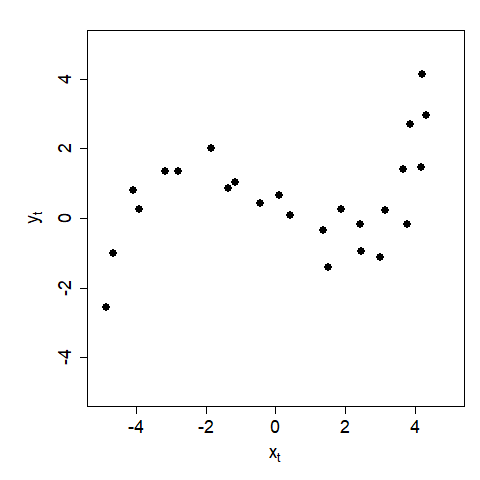
\includegraphics[width = \columnwidth]{Code2/autoco1.png}
	\end{minipage}
\hfill
	\begin{minipage}{0.48\columnwidth}
	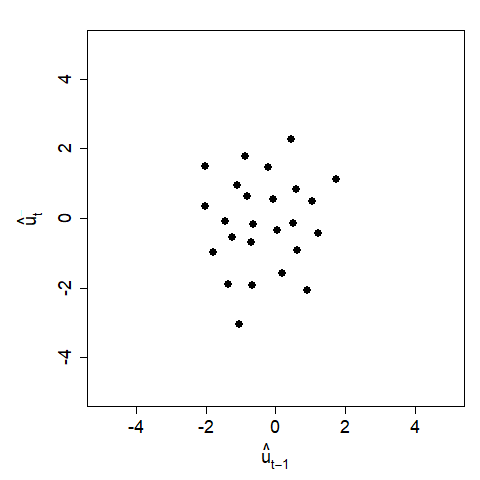
\includegraphics[width = \columnwidth]{Code2/autoco2.png}
	\end{minipage}
\end{figure}
\begin{figure}[H]
	\begin{minipage}{0.48\columnwidth}
		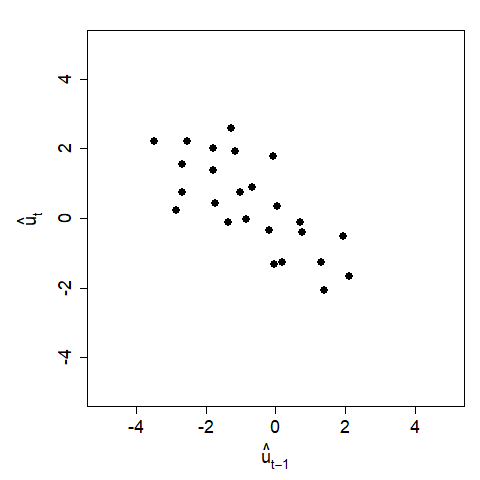
\includegraphics[width = \columnwidth]{Code2/autoco3.png}
	\end{minipage}
	\hfill
	\begin{minipage}{0.48\columnwidth}
		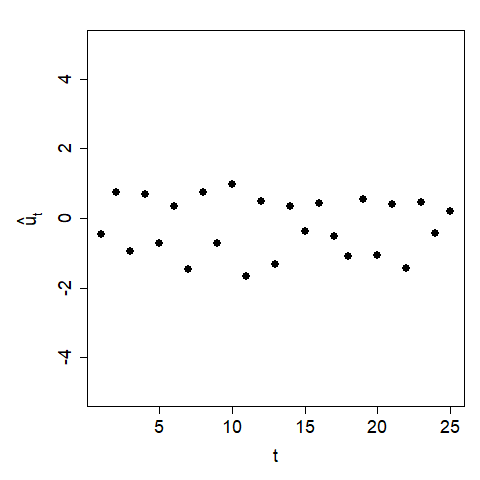
\includegraphics[width = \columnwidth]{Code2/autoco4.png}
	\end{minipage}
\end{figure}
\begin{figure}[H]
	\begin{minipage}{0.48\columnwidth}
		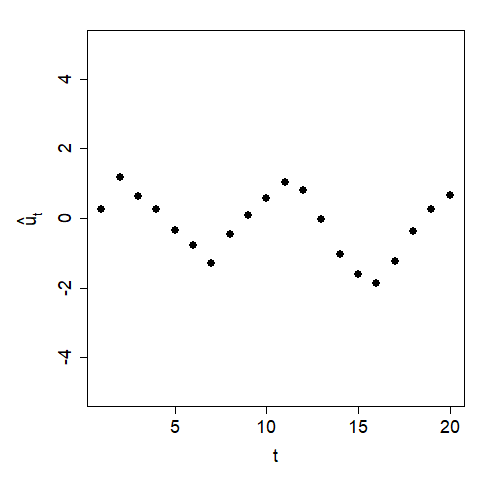
\includegraphics[width = \columnwidth]{Code2/autoco5.png}
	\end{minipage}
	\hfill
	\begin{minipage}{0.48\columnwidth}
		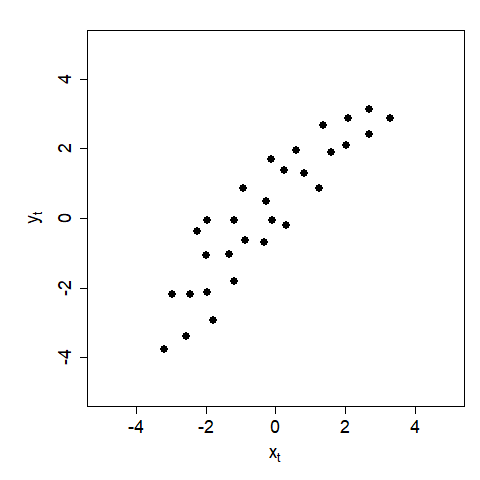
\includegraphics[width = \columnwidth]{Code2/autoco6.png}
	\end{minipage}
\end{figure}

\section*{\underline{Exercise 7}}

We estimate the parameters of a regression model
\[
	y_t = \beta_0 + \beta_1x_{1t} + \beta_2 x_{2t} + u_t 
\]by OLS using $T=15$ observations and obtain residuals $\hat{u}_t$:
\[
	4\quad3.5\quad3.5\quad2\quad-1\quad-4\quad-3\quad-2\quad-3\quad-1\quad1\quad3\quad1\quad-2\quad-2
\]
\begin{enumerate}[label = \alph*)]
	\item Plot pairs of residuals $(\hat{u}_{t-1};\hat{u}_t)$. Is there any evidence for positive, negative or no autocorrelation?
	\item Test your presumption in a) with a test for autocorrelation, assuming an AR(1) structure of error terms.
\end{enumerate}

\section*{\underline{Exercise 8}}
The figures below shows a histogram of $T=100$ residuals $\hat{u}_t$ obtained from an OLS regression. Additionally, some sums are given.
\begin{figure}[H]
	\centering
	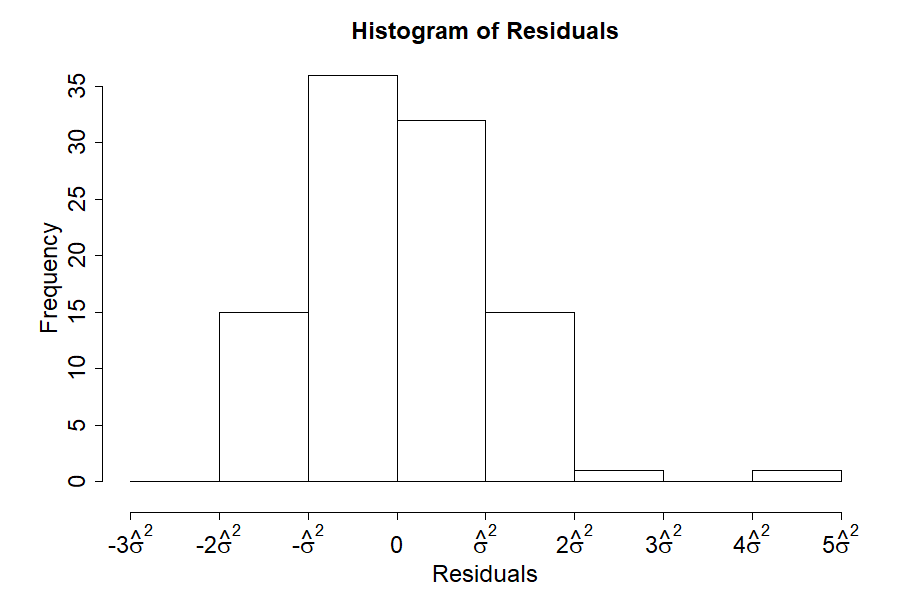
\includegraphics[width = 0.7\columnwidth]{Code2/hist8.png}
\end{figure}
\[
\frac{1}{100}\sum_{t = 1}^{100}{\hat{u}_t^2} = 0.2071 \qquad \frac{1}{100}\sum_{t = 1}^{100}{\hat{u}_t^3} = 0.0747 \qquad \frac{1}{100}\sum_{t = 1}^{100}{\hat{u}_t^4} = 0.1841
\]

\begin{enumerate}[label = \alph*)]
	\item Is there any evidence for the violation of assumption B4?
	\item Test your presumption in a) with a suitable test.
\end{enumerate}

\section*{\underline{Exercise 9}}
Proof the law of iterated expectation
\[
	\operatorname{E}\left(\operatorname{E}(X|Y)\right) = \operatorname{E}(X)\text{ ,}
\]where $X$ and $Y$ are continuous random variables with densities $f_X(x)$ and $f_Y(y)$ respectively.

\section*{\underline{Exercise 10}}
Consider the following macroeconomic model for $t = 1, ..., T$:
\begin{align*}
	C_t &= \beta_0 + \beta_1 Y_t + u_t\\
	Y_t &= C_t + I_t\\
	u_t &\overset{\text{iid}}{\sim} \mathcal{N}(0, \sigma_u^2)\\
	\operatorname{Cov}(I_t, u_t) &= 0 \qquad \forall t=1,...,T
\end{align*}

where $C = (C_1,...,C_T)'$ denotes consumption, $Y = (Y_1,...,Y_T)'$ the income and $I = (I_1, ..., I_T)'$ investments. With $\mathds{1}$, a vector of ones, the following matrix is calculated:

\[
\begin{pmatrix}
	\mathds{1}' \\ 
	C' \\ 
	Y' \\ 
	I'
\end{pmatrix}
\begin{pmatrix}
\mathds{1} & C & Y & I
\end{pmatrix}
=
\begin{pmatrix}
	9 & 3905.7 & 4007.6 & 101.9 \\ 
	3905.7 & 1695841.58 & 1740366.94 & 44525.36 \\ 
	4007.6 & 1740366.94 & 1786149.92 & 45782.98 \\ 
	101.9 & 44525.36 & 45782.98 & 1257.62%
\end{pmatrix}%
\]

\begin{enumerate}[label = \alph*)]
	\item Why is an OLS estimation not justified in this situation?
	\item Perform an IV estimation of the parameter vector. Use $I_t$ as an instrument for $Y_t$.
	\item What requirements are needed for an instrument to achieve a consistent estimation?
\end{enumerate}


\section*{\underline{Exercise 11}}

To investigate if a price increase can reduce cigarette consumption, you have yearly data of 48 states of the US for 1985 to 1995. You are interested in estimating the model
\[
\ln\left(\frac{y_{i; 1995}}{y_{i; 1985}}\right) = \alpha + \beta_1\ln\left(\frac{x_{i; 1995}}{x_{i; 1985}}\right) + \beta_2\ln\left(\frac{w_{i; 1995}}{w_{i; 1985}}\right) + u_i 
\]
where $y_{i; j}$ denotes cigarette consumption of state $i$ in the year $j$ (in packs per person), $x_{i; j}$ the price of cigarettes (including taxes) and $w_{i; j}$ the real income per person.\\
Further you have data for mean real tobacco tax load $z1_{i;j}$ and mean real excise duties $z2_{i;j}$\footnote{the average tax due to the broad-based state sales tax applied to all consumption goods.}. Both variables $z1$ and $z2$ are measured in cents per pack.\\
Income $w_{i; j}$ is assumed to be contemporarily uncorrelated to the error term and can thus be used as exogenous variable.

\begin{enumerate}[label = \alph*)]
	\item Calculate OLS estimates for the model above.
	\[\hspace{-1cm}
		(\mathbf{X}'\mathbf{X})^{-1}=%
		\begin{bmatrix}
		1.4665 & -1.4744 & -1.0659 \\ 
		-1.4744 & 2.6917 & -0.082 \\ 
		-1.0659 & -0.082 & 1.9366%
		\end{bmatrix}%
		,\qquad \mathbf{X}'\mathbf{y}=%
		\begin{bmatrix}
		-12.0695 \\ 
		-7.2261 \\ 
		-7.0925%
		\end{bmatrix}%
		,\qquad \widehat{\mathbf{u}}'\widehat{\mathbf{u}}=0.34884.
	\]
	\item Discuss if OLS is a justified method for the estimation of parameters in this case.
	\item Can $z2$ be used to obtain a valid instrument for the cigarette price $x$? Give reasons for your answer.
	\item Perform an IV estimation by using $\ln(z2)$ as instrument for $\ln(x)$. Estimate the variance matrix of the obtained estimator $\hat{\beta}_{\text{IV}1}$.
	\[
		(\mathbf{Z}_1'\mathbf{X})^{-1}=%
		\begin{bmatrix}
		1.0631 & -0.7733 & -1.0762 \\ 
		-0.7379 & 1.4117 & -0.0634 \\ 
		-1.0884 & -0.0430 & 1.9361%
		\end{bmatrix}%
		,\qquad \mathbf{Z}_1'\mathbf{y}=%
		\begin{bmatrix}
		-12.0695 \\ 
		-7.5505 \\ 
		-7.0925%
		\end{bmatrix}%
	\]
	\[
	(\mathbf{X}'%
	\mathbf{Z}_1(\mathbf{Z}_1'\mathbf{Z}_1)^{-1}\mathbf{Z%
	}_1'\mathbf{X})^{-1}=%
	\begin{bmatrix}
	1.7501 & -1.9921 & -1.0502 \\ 
	-1.9921 & 3.6367 & -0.1108 \\ 
	-1.0502 & -0.1108 & 1.9375%
	\end{bmatrix}%
	,\qquad \widehat{\mathbf{u}}_1'\widehat{\mathbf{u}}_1=0.36844,
	\]
	\item Test the contemporary correlation between $\ln\left(\frac{x_{i;1995}}{x_{i;1985}}\right)$ and $u_i$ using a 5\% level of significance.
	\item Repeat the IV estimation, but this time also include $\ln(z1)$ as an instrument for $ln(x)$. Compute the variance matrix estimator $\widehat{\operatorname{Var}}\left(\hat{\beta}_{\text{IV}2}\right)$.
	\[
	(\mathbf{X}'\mathbf{P}\mathbf{X})^{-1}=%
	\begin{bmatrix}
	1.7237 & -1.9440 & -1.0516 \\ 
	-1.9440 & 3.5489 & -0.1081 \\ 
	-1.0516 & -0.1081 & 1.9374%
	\end{bmatrix}%
	,\qquad \mathbf{X}'\mathbf{P}\mathbf{y}=%
	\begin{bmatrix}
	-12.0695 \\ 
	-7.1749 \\ 
	-7.0925%
	\end{bmatrix}%
	\]\[
	\widehat{\mathbf{u}}'\widehat{\mathbf{u}}=0.35834.
	\qquad \mathbf{P} = \mathbf{Z}_2(\mathbf{Z}_2'\mathbf{Z}_2)^{-1}\mathbf{Z}_2'
	\]
	\item Which of the two models would you prefer? Give reasons for your answer.
	\item What is your conclusion regarding the question at the beginning?
\end{enumerate}


%\begin{enumerate}
%	\item[g)] Pr\"{u}fen Sie zum Signifikanzniveau $\alpha =5\%$, ob die beiden
%	Instrumente $\ln z1$ und $\ln z2$ exogen (d.h. nicht mit der St\"{o}rgr\"{o}%
%	\ss e $u$ korreliert) sind. Hierf\"{u}r nutzen Sie die Summen der
%	Residuenquadrate aus der Sch\"{a}tzung der folgenden Regression:%
%	\begin{equation*}
%	\widehat{\widetilde{u}}=\delta _{0}+\delta _{1}(\ln z1_{i,1995}-\ln
%	z1_{i,1985})+\delta _{2}(\ln z2_{i,1995}-\ln z2_{i,1985})+\delta _{3}(\ln
%	w_{i,1995}-\ln w_{i,1985})+e_{i}
%	\end{equation*}%
%	\begin{equation*}
%	S_{\widehat{e}\widehat{e}}=0.30294
%	\end{equation*}%
%	und diese aus der Sch\"{a}tzung des restringierten Modells:%
%	\begin{equation*}
%	\widehat{\widetilde{u}}=\delta _{0}+\delta _{3}(\ln w_{i,1995}-\ln
%	w_{i,1985})+e_{i}^{0}
%	\end{equation*}%
%	\begin{equation*}
%	S_{\widehat{e}\widehat{e}}^{0}=0.35835.
%	\end{equation*}%
%	Hinweis: The overidentifying restrictions test, $J$-Statistic in Stock and
%	Watson.
%\end{enumerate}

\section*{\underline{Exercise 12}}

The following figure shows data from 1995 to 2005, including the total net income in billion TNI ($x_t$) and the total number of private bankruptcies ($y_t$) in Germany.
\begin{figure}[H]
	\centering
	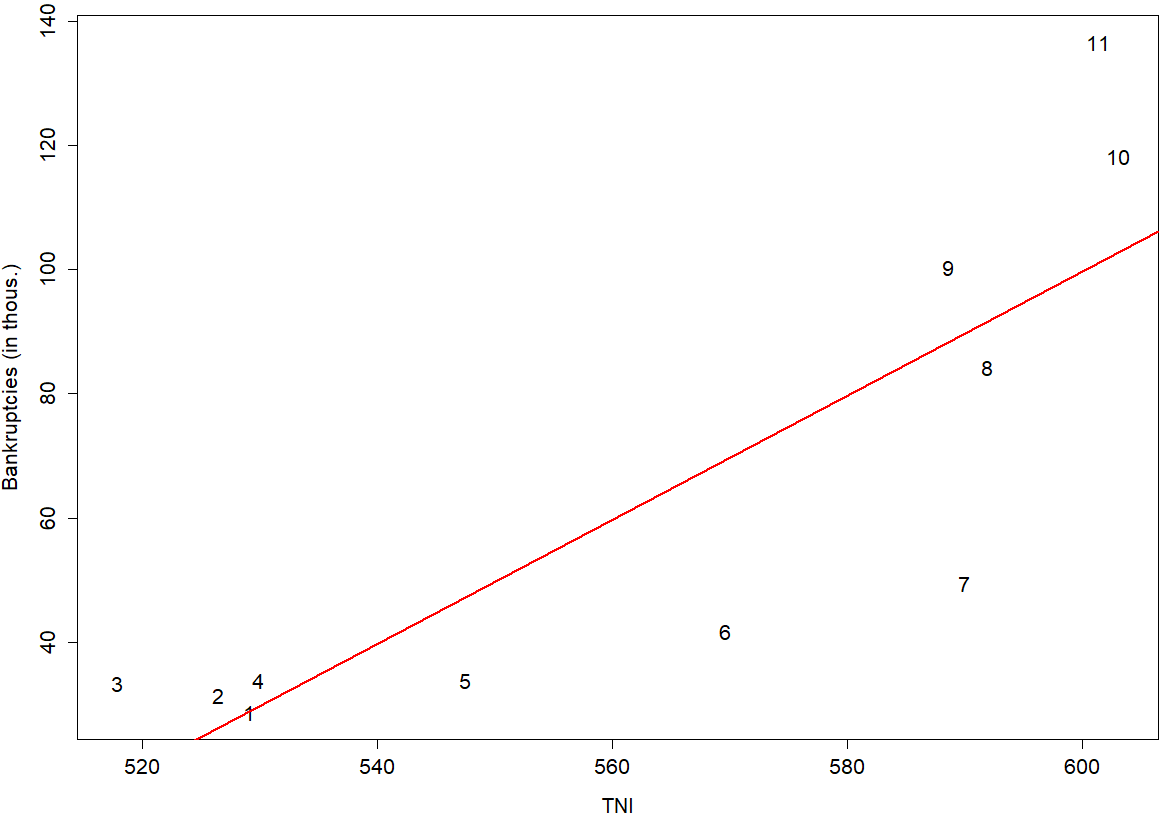
\includegraphics[width = 0.7\columnwidth]{Code2/insolvenzen.png}
\end{figure}
The parameters of the regression model are estimated as
\[
	\hat{y}_t = -498\hphantom{i}800.2 + 997.4 x_t
\]with a sum of squared residuals $S_{\hat{u}\hat{u}}^{\text{0}} = 4\hphantom{i}540\hphantom{i}767\hphantom{i}881$.
\begin{enumerate}[label = \alph*)]
	\item At the end of 2001 a new law simplified the insolvency filing. Try to guess where a structural break in the data might be.
	\item With the help of dummy variables, set up a regression model, that takes a structural break into account. Sketch the regressor matrix $X$.
	\item The above model is estimated:
	\begin{align*}
		\hat{y}_t =& -99\hphantom{i}604.64 - 1\hphantom{i}287\hphantom{i}453.9 D_t + 249.32 x_t + 2\hphantom{i}261.3 D_t x_t \\
		&\hphantom{M}(79\hphantom{i} 061.3)\hphantom{MM} (462\hphantom{i} 758.5) \hphantom{MM}(145.1)\hphantom{MM} (778.3)\\
		S_{\hat{u}\hat{u}}^{\text{SB}} =& 617\hphantom{i}588\hphantom{i}408
	\end{align*}
	Use the F-test to test for a structural break at a 5\% level.
	\item Separate regression in the two subgroups yields following results. Fill in the blank spaces and compare with c).
	\begin{align*}
	\hat{y}_t^I =&\hphantom{i} -99\hphantom{i} 604.64 + 249.32 x_t\\
	&\hphantom{i}(24 \hphantom{i}769.34)\hphantom{MM} (45.46)\\
	S_{\hat{u}\hat{u}}^I =&\hphantom{i} 43 \hphantom{i}298\hphantom{i} 384\\
	\hat{y}_t^{II} =&\hphantom{i} \rule{3cm}{1pt} + \rule{3cm}{1pt} x_t\\
	&\hphantom{iM} (822\hphantom{i}568) \hphantom{MMMMM}(1\hphantom{i}380)\\
	S_{\hat{u}\hat{u}}^{II} =&\hphantom{i} \rule{3cm}{1pt}
	\end{align*}
\end{enumerate}

\section*{\underline{Exercise 13}}
The amount of ice cream sold in a month $q_t$ shall be explained by the price $p_t$, the expenses for advertisement $x_t$ and dummy variables indicating early, main and late season in an inhomogeneous regression model. The dummy variables are defined as
\[
	D_{1,t} = \begin{cases}1 &\text{if }t\text{ is a month from January and April}\\
	0&\text{else} \end{cases}
\]and accordingly $D_{2,t}$ for the months May to August and $D_{3, t}$ from September to December. Data is available for the months Jan.1997 to May 2000.
\begin{enumerate}[label = \alph*)]
\item Formulate a suitable regression model for the amount of ice cream sold. Is it reasonable to include every dummy variable in the model? Review critically.
\item The following regression was performed
\begin{align*}
	\hat{q}_t &= 2237.58 - 575.99 p_t + 0.13 x_t + 440.4 D_{2, t} + 22.6 D_{3, t}\\
	&\hphantom{M}(591.55)\hphantom{M}(218.26)\hphantom{M}(0.04)\hphantom{MM}(70.92)\hphantom{Mi}(61.59)\\
	R^2 &= 0.778\hphantom{MMMM} \bar{R}^2 = 0.754
\end{align*}
\begin{enumerate}
	\item[i)] Comment the sign of estimated coefficients.
	\item[ii)] Test if the turnover in the main season differs significantly from turnover in early season. (5\% level)
\end{enumerate}	
\end{enumerate}
\newpage
\section*{\underline{Exercise 14}}
Consider the data from following plot
\begin{figure}[H]
	\centering
	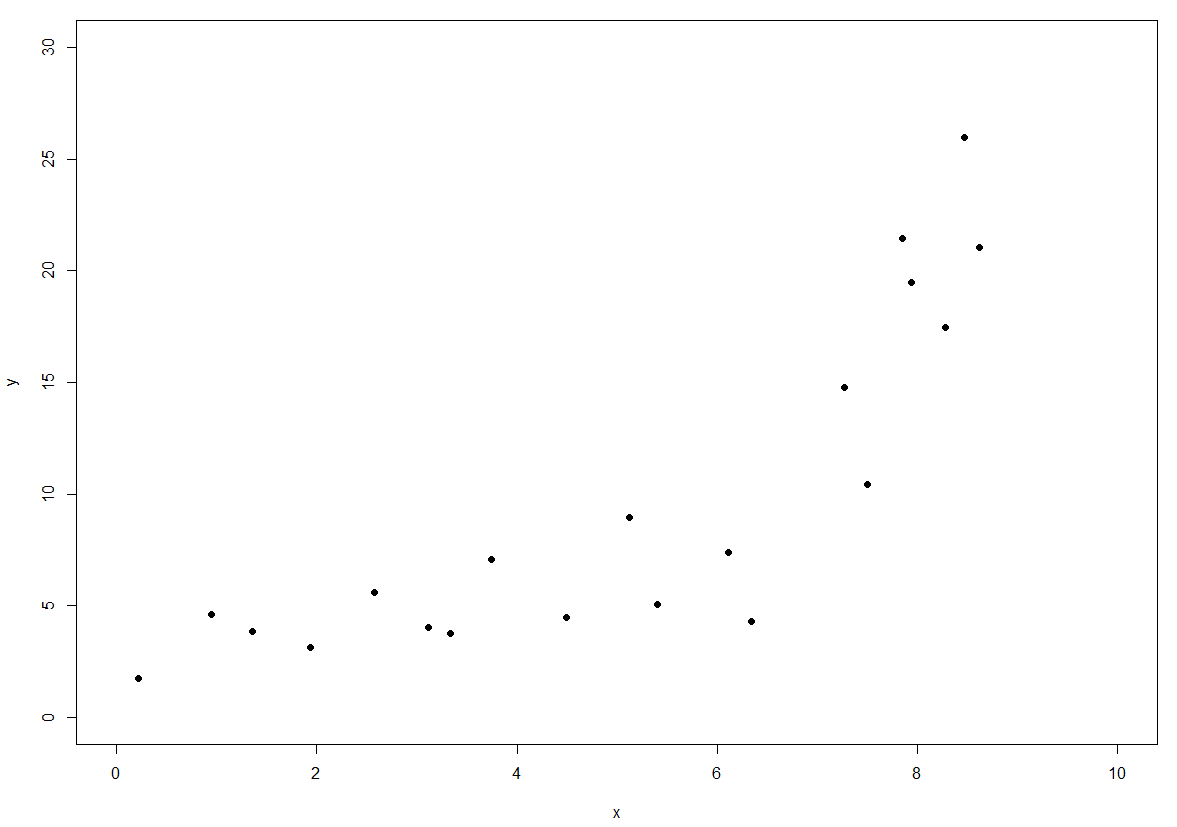
\includegraphics[width = 0.7\columnwidth]{Code2/sbreak1.png}
\end{figure}
You are interested in testing for a structural break.
\begin{enumerate}[label = \alph*)]
	\item Only from visual impression, where would you suspect the break?
	\item You separate the data into two groups, where $T_1$ shall denote the largest index belonging to group 1. You perform an OLS regression on the whole sample, giving $S_{\hat{u}\hat{u}}$ and for $T_1 = 3,...,17$ you perform separate OLS regressions, which yields sums of squares residuals $S_{\hat{u}\hat{u}}^I$ and $S_{\hat{u}\hat{u}}^{II}$.
	\begin{table}[H]
		\centering
		\resizebox{0.95\columnwidth}{!}{\begin{tabular}{c|ccccccccccccccc}
			\toprule
			$T_1$&3 & 4 & 5 & 6 & 7 & 8 & 9 & 10 & 11 & 12 & 13 & 14 & 15&16&17\\
			\midrule
			$S_{\hat{u}\hat{u}}^I$ & 1.5 & 3.6 & 4.1 & 5.6 & 6.5 & 10.0 & 11.8 & 17.8 & 21.2 & 21.3 & 28.6 & 70.5 & 71.2 & 172.8 & 210.8 \\ 
			$S_{\hat{u}\hat{u}}^{II}$ & 262.9 & 249.6 & 220.5 & 209.8 & 199.1 & 150.1 & 139.4 & 94.7 & 80.8 & 71.0 & 69.5 & 65.3 & 36.0 & 31.1 & 28.3 \\ 
			Tstat & 1.9 & 2.3 & 3.6 & 4.1 & 4.7 & 8.3 & 9.3 & 15.2 & 17.6 & 20.3 & 18.6 & 11.2 & 16.3 & 4.8 & 2.9 \\
			\bottomrule
		\end{tabular}}
	\end{table}
	\begin{enumerate}[label = \roman*)]
		\item How were the test statistics in the table computed?
		\item Where would suspect a structural break now given the table?
		\item Would your suggestion(s) for structural breaks in a) and ii) be significant at a 5\% level?
		\item If you wanted to complete the table for remaining possible values of $T_1$, how would you calculate a test statistic and what would be its distribution under the null hypothesis of no structural break?
	\end{enumerate}
	\item Could you perform the above investigation if you hat two exogenous variables and an intercept? Sketch the steps you would take.
	\item Is there an other way of dealing with above data besides modeling a structural break?
\end{enumerate} 


\section*{\underline{Exercise 15}}
Consider a bivariate dynamic model with four lags in $x$:
\begin{equation*}
y_{t}=0.55\left(
0.02x_{t}+0.15x_{t-1}+0.43x_{t-2}+0.23x_{t-3}+0.17x_{t-4}\right) +u_{t}.
\end{equation*}
Compute the short run and long run multiplier for given model.

\section*{\underline{Exercise 16}}
The monthly sales turnover of a product is modeled using the dynamic model
\[
	S_t = \alpha + \beta_0A_t + \beta_1A_{t-1} + .... + u_t
\]where $A_t$ is the advertising expenses in month $t$ and $u_t\sim\mathcal{N}(0, \sigma^2)$. You assume that the coefficients $\beta_i$ decay geometrically starting from $\beta_2$, so that $\beta_k = \lambda^{k-1}\beta_1$ for $k = 2,3,...$, where $0\le \lambda < 1$.
\begin{enumerate}
	\item Perform the Koyck transformation and explain why an OLS estimation is not justified in this situation.
	\item How would you estimate the parameters of the model?
	\item The estimation gives
	\[
		\hat{S}_t = 286.3 + 0.127A_t + 0.081A_{t-1} + 0.399S_{t-1}
	\]Compute the estimates for $\lambda$, $\alpha$, $\beta_0$, $\beta_1$ and $\beta_k$ ($k$ = 2,3,...).
\end{enumerate}

\newpage
\begin{table}[ht]
	\centering
	\resizebox{\columnwidth}{!}{\begin{tabular}{>{\bfseries}rd{1.3}d{1.3}d{1.3}d{2.3}d{2.3}|>{\bfseries}rd{1.3}d{1.3}d{1.3}d{2.3}d{2.3}}
			\toprule
			\toprule
			df  & \multicolumn{1}{c}{90\%} & \multicolumn{1}{c}{92.5\%} & \multicolumn{1}{c}{95\%} & \multicolumn{1}{c}{97.5\%} & \multicolumn{1}{c}{99\%} & df  & \multicolumn{1}{c}{90\%} & \multicolumn{1}{c}{92.5\%} & \multicolumn{1}{c}{95\%} & \multicolumn{1}{c}{97.5\%} & \multicolumn{1}{c}{99\%} \\
			\midrule
			1 & 3.078 & 4.165 & 6.314 & 12.706 & 31.821 &  51 & 1.298 & 1.462 & 1.675 & 2.008 & 2.402  \\ 
			2 & 1.886 & 2.282 & 2.920 & 4.303 & 6.965 &  52 & 1.298 & 1.461 & 1.675 & 2.007 & 2.400   \\ 
			3 & 1.638 & 1.924 & 2.353 & 3.182 & 4.541 &  53 & 1.298 & 1.461 & 1.674 & 2.006 & 2.399   \\ 
			4 & 1.533 & 1.778 & 2.132 & 2.776 & 3.747 & 54 & 1.297 & 1.460 & 1.674 & 2.005 & 2.397  \\ 
			5 & 1.476 & 1.699 & 2.015 & 2.571 & 3.365 & 55 & 1.297 & 1.460 & 1.673 & 2.004 & 2.396   \\ 
			6 & 1.440 & 1.650 & 1.943 & 2.447 & 3.143 & 56 & 1.297 & 1.460 & 1.673 & 2.003 & 2.395   \\ 
			7 & 1.415 & 1.617 & 1.895 & 2.365 & 2.998 & 57 & 1.297 & 1.459 & 1.672 & 2.002 & 2.394   \\ 
			8 & 1.397 & 1.592 & 1.860 & 2.306 & 2.896 & 58 & 1.296 & 1.459 & 1.672 & 2.002 & 2.392  \\ 
			9 & 1.383 & 1.574 & 1.833 & 2.262 & 2.821 & 59 & 1.296 & 1.459 & 1.671 & 2.001 & 2.391   \\ 
			10 & 1.372 & 1.559 & 1.812 & 2.228 & 2.764 & 60 & 1.296 & 1.458 & 1.671 & 2.000 & 2.390   \\ 
			11 & 1.363 & 1.548 & 1.796 & 2.201 & 2.718 & 61 & 1.296 & 1.458 & 1.670 & 2.000 & 2.389   \\ 
			12 & 1.356 & 1.538 & 1.782 & 2.179 & 2.681 & 62 & 1.295 & 1.458 & 1.670 & 1.999 & 2.388   \\ 
			13 & 1.350 & 1.530 & 1.771 & 2.160 & 2.650 & 63 & 1.295 & 1.457 & 1.669 & 1.998 & 2.387   \\ 
			14 & 1.345 & 1.523 & 1.761 & 2.145 & 2.624 & 64 & 1.295 & 1.457 & 1.669 & 1.998 & 2.386   \\ 
			15 & 1.341 & 1.517 & 1.753 & 2.131 & 2.602 & 65 & 1.295 & 1.457 & 1.669 & 1.997 & 2.385   \\ 
			16 & 1.337 & 1.512 & 1.746 & 2.120 & 2.583 & 66 & 1.295 & 1.456 & 1.668 & 1.997 & 2.384  \\ 
			17 & 1.333 & 1.508 & 1.740 & 2.110 & 2.567 & 67 & 1.294 & 1.456 & 1.668 & 1.996 & 2.383  \\ 
			18 & 1.330 & 1.504 & 1.734 & 2.101 & 2.552 & 68 & 1.294 & 1.456 & 1.668 & 1.995 & 2.382   \\ 
			19 & 1.328 & 1.500 & 1.729 & 2.093 & 2.539 & 69 & 1.294 & 1.456 & 1.667 & 1.995 & 2.382  \\ 
			20 & 1.325 & 1.497 & 1.725 & 2.086 & 2.528 & 70 & 1.294 & 1.456 & 1.667 & 1.994 & 2.381  \\ 
			21 & 1.323 & 1.494 & 1.721 & 2.080 & 2.518 & 71 & 1.294 & 1.455 & 1.667 & 1.994 & 2.380  \\ 
			22 & 1.321 & 1.492 & 1.717 & 2.074 & 2.508 & 72 & 1.293 & 1.455 & 1.666 & 1.993 & 2.379   \\ 
			23 & 1.319 & 1.489 & 1.714 & 2.069 & 2.500 & 73 & 1.293 & 1.455 & 1.666 & 1.993 & 2.379   \\ 
			24 & 1.318 & 1.487 & 1.711 & 2.064 & 2.492 & 74 & 1.293 & 1.455 & 1.666 & 1.993 & 2.378   \\ 
			25 & 1.316 & 1.485 & 1.708 & 2.060 & 2.485 & 75 & 1.293 & 1.454 & 1.665 & 1.992 & 2.377  \\ 
			26 & 1.315 & 1.483 & 1.706 & 2.056 & 2.479 & 76 & 1.293 & 1.454 & 1.665 & 1.992 & 2.376   \\ 
			27 & 1.314 & 1.482 & 1.703 & 2.052 & 2.473 & 77 & 1.293 & 1.454 & 1.665 & 1.991 & 2.376   \\ 
			28 & 1.313 & 1.480 & 1.701 & 2.048 & 2.467 & 78 & 1.292 & 1.454 & 1.665 & 1.991 & 2.375   \\ 
			29 & 1.311 & 1.479 & 1.699 & 2.045 & 2.462 & 79 & 1.292 & 1.454 & 1.664 & 1.990 & 2.374   \\ 
			30 & 1.310 & 1.477 & 1.697 & 2.042 & 2.457 & 80 & 1.292 & 1.453 & 1.664 & 1.990 & 2.374   \\ 
			31 & 1.309 & 1.476 & 1.696 & 2.040 & 2.453 & 81 & 1.292 & 1.453 & 1.664 & 1.990 & 2.373  \\ 
			32 & 1.309 & 1.475 & 1.694 & 2.037 & 2.449 & 82 & 1.292 & 1.453 & 1.664 & 1.989 & 2.373   \\ 
			33 & 1.308 & 1.474 & 1.692 & 2.035 & 2.445 & 83 & 1.292 & 1.453 & 1.663 & 1.989 & 2.372  \\ 
			34 & 1.307 & 1.473 & 1.691 & 2.032 & 2.441 & 84 & 1.292 & 1.453 & 1.663 & 1.989 & 2.372   \\ 
			35 & 1.306 & 1.472 & 1.690 & 2.030 & 2.438 & 85 & 1.292 & 1.453 & 1.663 & 1.988 & 2.371   \\ 
			36 & 1.306 & 1.471 & 1.688 & 2.028 & 2.434 & 86 & 1.291 & 1.453 & 1.663 & 1.988 & 2.370   \\ 
			37 & 1.305 & 1.470 & 1.687 & 2.026 & 2.431 & 87 & 1.291 & 1.452 & 1.663 & 1.988 & 2.370   \\ 
			38 & 1.304 & 1.469 & 1.686 & 2.024 & 2.429 & 88 & 1.291 & 1.452 & 1.662 & 1.987 & 2.369   \\ 
			39 & 1.304 & 1.468 & 1.685 & 2.023 & 2.426 & 89 & 1.291 & 1.452 & 1.662 & 1.987 & 2.369  \\ 
			40 & 1.303 & 1.468 & 1.684 & 2.021 & 2.423 & 90 & 1.291 & 1.452 & 1.662 & 1.987 & 2.368   \\ 
			41 & 1.303 & 1.467 & 1.683 & 2.020 & 2.421 & 91 & 1.291 & 1.452 & 1.662 & 1.986 & 2.368   \\ 
			42 & 1.302 & 1.466 & 1.682 & 2.018 & 2.418 & 92 & 1.291 & 1.452 & 1.662 & 1.986 & 2.368  \\ 
			43 & 1.302 & 1.466 & 1.681 & 2.017 & 2.416 & 93 & 1.291 & 1.452 & 1.661 & 1.986 & 2.367  \\ 
			44 & 1.301 & 1.465 & 1.680 & 2.015 & 2.414 & 94 & 1.291 & 1.451 & 1.661 & 1.986 & 2.367   \\ 
			45 & 1.301 & 1.465 & 1.679 & 2.014 & 2.412 & 95 & 1.291 & 1.451 & 1.661 & 1.985 & 2.366   \\ 
			46 & 1.300 & 1.464 & 1.679 & 2.013 & 2.410 & 96 & 1.290 & 1.451 & 1.661 & 1.985 & 2.366   \\ 
			47 & 1.300 & 1.463 & 1.678 & 2.012 & 2.408 & 97 & 1.290 & 1.451 & 1.661 & 1.985 & 2.365  \\ 
			48 & 1.299 & 1.463 & 1.677 & 2.011 & 2.407 & 98 & 1.290 & 1.451 & 1.661 & 1.984 & 2.365 \\ 
			49 & 1.299 & 1.462 & 1.677 & 2.010 & 2.405 & 99 & 1.290 & 1.451 & 1.660 & 1.984 & 2.365   \\ 
			50 & 1.299 & 1.462 & 1.676 & 2.009 & 2.403 & $\boldsymbol{\infty}$ & 1.282 & 1.440 & 1.645 & 1.960 & 2.326   \\ 
			\bottomrule
			\bottomrule
	\end{tabular}}
	\caption{Quantiles of $t$-distribution}
\end{table}

\newpage
\begin{landscape}
\begin{table}[ht]
	\centering
	\resizebox{\columnwidth}{!}{
		\begin{tabular}{rd{2.2}d{2.2}d{2.2}d{2.2}d{2.2}d{2.2}d{2.2}d{2.2}d{2.2}d{2.2}d{2.2}d{2.2}d{2.2}d{2.2}d{2.2}d{2.2}d{2.2}d{2.2}d{2.2}d{2.2}d{2.2}d{2.2}d{2.2}d{2.2}d{2.2}d{2.2}d{2.2}d{2.2}d{2.2}d{2.2}d{2.2}d{2.2}d{2.2}d{2.2}d{2.2}d{2.2}}
		\toprule
		\toprule
		Z $\rightarrow$ & \multicolumn{1}{c}{2} & \multicolumn{1}{c}{3} & \multicolumn{1}{c}{4} & \multicolumn{1}{c}{5} & \multicolumn{1}{c}{6} & \multicolumn{1}{c}{7} & \multicolumn{1}{c}{8} & \multicolumn{1}{c}{9} & \multicolumn{1}{c}{10} & \multicolumn{1}{c}{11} & \multicolumn{1}{c}{12} & \multicolumn{1}{c}{13} & \multicolumn{1}{c}{14} & \multicolumn{1}{c}{15} & \multicolumn{1}{c}{16} & \multicolumn{1}{c}{17} & \multicolumn{1}{c}{18} & \multicolumn{1}{c}{19} & \multicolumn{1}{c}{20} & \multicolumn{1}{c}{21} & \multicolumn{1}{c}{22} & \multicolumn{1}{c}{23} & \multicolumn{1}{c}{24} & \multicolumn{1}{c}{25} & \multicolumn{1}{c}{26} & \multicolumn{1}{c}{27} & \multicolumn{1}{c}{28} & \multicolumn{1}{c}{29} & \multicolumn{1}{c}{30} & \multicolumn{1}{c}{40} & \multicolumn{1}{c}{50} & \multicolumn{1}{c}{60} & \multicolumn{1}{c}{70} & \multicolumn{1}{c}{80} & \multicolumn{1}{c}{90} & \multicolumn{1}{c}{100} \\ 
		\midrule
		N$\downarrow$\hphantom{M}2 & 19.00 & 19.16 & 19.25 & 19.30 & 19.33 & 19.35 & 19.37 & 19.38 & 19.40 & 19.40 & 19.41 & 19.42 & 19.42 & 19.43 & 19.43 & 19.44 & 19.44 & 19.44 & 19.45 & 19.45 & 19.45 & 19.45 & 19.45 & 19.46 & 19.46 & 19.46 & 19.46 & 19.46 & 19.46 & 19.47 & 19.48 & 19.48 & 19.48 & 19.48 & 19.48 & 19.49 \\ 
		3 & 9.55 & 9.28 & 9.12 & 9.01 & 8.94 & 8.89 & 8.85 & 8.81 & 8.79 & 8.76 & 8.74 & 8.73 & 8.71 & 8.70 & 8.69 & 8.68 & 8.67 & 8.67 & 8.66 & 8.65 & 8.65 & 8.64 & 8.64 & 8.63 & 8.63 & 8.63 & 8.62 & 8.62 & 8.62 & 8.59 & 8.58 & 8.57 & 8.57 & 8.56 & 8.56 & 8.55 \\ 
		4 & 6.94 & 6.59 & 6.39 & 6.26 & 6.16 & 6.09 & 6.04 & 6.00 & 5.96 & 5.94 & 5.91 & 5.89 & 5.87 & 5.86 & 5.84 & 5.83 & 5.82 & 5.81 & 5.80 & 5.79 & 5.79 & 5.78 & 5.77 & 5.77 & 5.76 & 5.76 & 5.75 & 5.75 & 5.75 & 5.72 & 5.70 & 5.69 & 5.68 & 5.67 & 5.67 & 5.66 \\ 
		5 & 5.79 & 5.41 & 5.19 & 5.05 & 4.95 & 4.88 & 4.82 & 4.77 & 4.74 & 4.70 & 4.68 & 4.66 & 4.64 & 4.62 & 4.60 & 4.59 & 4.58 & 4.57 & 4.56 & 4.55 & 4.54 & 4.53 & 4.53 & 4.52 & 4.52 & 4.51 & 4.50 & 4.50 & 4.50 & 4.46 & 4.44 & 4.43 & 4.42 & 4.41 & 4.41 & 4.41 \\ 
		6 & 5.14 & 4.76 & 4.53 & 4.39 & 4.28 & 4.21 & 4.15 & 4.10 & 4.06 & 4.03 & 4.00 & 3.98 & 3.96 & 3.94 & 3.92 & 3.91 & 3.90 & 3.88 & 3.87 & 3.86 & 3.86 & 3.85 & 3.84 & 3.83 & 3.83 & 3.82 & 3.82 & 3.81 & 3.81 & 3.77 & 3.75 & 3.74 & 3.73 & 3.72 & 3.72 & 3.71 \\ 
		7 & 4.74 & 4.35 & 4.12 & 3.97 & 3.87 & 3.79 & 3.73 & 3.68 & 3.64 & 3.60 & 3.57 & 3.55 & 3.53 & 3.51 & 3.49 & 3.48 & 3.47 & 3.46 & 3.44 & 3.43 & 3.43 & 3.42 & 3.41 & 3.40 & 3.40 & 3.39 & 3.39 & 3.38 & 3.38 & 3.34 & 3.32 & 3.30 & 3.29 & 3.29 & 3.28 & 3.27 \\ 
		8 & 4.46 & 4.07 & 3.84 & 3.69 & 3.58 & 3.50 & 3.44 & 3.39 & 3.35 & 3.31 & 3.28 & 3.26 & 3.24 & 3.22 & 3.20 & 3.19 & 3.17 & 3.16 & 3.15 & 3.14 & 3.13 & 3.12 & 3.12 & 3.11 & 3.10 & 3.10 & 3.09 & 3.08 & 3.08 & 3.04 & 3.02 & 3.01 & 2.99 & 2.99 & 2.98 & 2.97 \\ 
		9 & 4.26 & 3.86 & 3.63 & 3.48 & 3.37 & 3.29 & 3.23 & 3.18 & 3.14 & 3.10 & 3.07 & 3.05 & 3.03 & 3.01 & 2.99 & 2.97 & 2.96 & 2.95 & 2.94 & 2.93 & 2.92 & 2.91 & 2.90 & 2.89 & 2.89 & 2.88 & 2.87 & 2.87 & 2.86 & 2.83 & 2.80 & 2.79 & 2.78 & 2.77 & 2.76 & 2.76 \\ 
		10 & 4.10 & 3.71 & 3.48 & 3.33 & 3.22 & 3.14 & 3.07 & 3.02 & 2.98 & 2.94 & 2.91 & 2.89 & 2.86 & 2.85 & 2.83 & 2.81 & 2.80 & 2.79 & 2.77 & 2.76 & 2.75 & 2.75 & 2.74 & 2.73 & 2.72 & 2.72 & 2.71 & 2.70 & 2.70 & 2.66 & 2.64 & 2.62 & 2.61 & 2.60 & 2.59 & 2.59 \\ 
		11 & 3.98 & 3.59 & 3.36 & 3.20 & 3.09 & 3.01 & 2.95 & 2.90 & 2.85 & 2.82 & 2.79 & 2.76 & 2.74 & 2.72 & 2.70 & 2.69 & 2.67 & 2.66 & 2.65 & 2.64 & 2.63 & 2.62 & 2.61 & 2.60 & 2.59 & 2.59 & 2.58 & 2.58 & 2.57 & 2.53 & 2.51 & 2.49 & 2.48 & 2.47 & 2.46 & 2.46 \\ 
		12 & 3.89 & 3.49 & 3.26 & 3.11 & 3.00 & 2.91 & 2.85 & 2.80 & 2.75 & 2.72 & 2.69 & 2.66 & 2.64 & 2.62 & 2.60 & 2.58 & 2.57 & 2.56 & 2.54 & 2.53 & 2.52 & 2.51 & 2.51 & 2.50 & 2.49 & 2.48 & 2.48 & 2.47 & 2.47 & 2.43 & 2.40 & 2.38 & 2.37 & 2.36 & 2.36 & 2.35 \\ 
		13 & 3.81 & 3.41 & 3.18 & 3.03 & 2.92 & 2.83 & 2.77 & 2.71 & 2.67 & 2.63 & 2.60 & 2.58 & 2.55 & 2.53 & 2.51 & 2.50 & 2.48 & 2.47 & 2.46 & 2.45 & 2.44 & 2.43 & 2.42 & 2.41 & 2.41 & 2.40 & 2.39 & 2.39 & 2.38 & 2.34 & 2.31 & 2.30 & 2.28 & 2.27 & 2.27 & 2.26 \\ 
		14 & 3.74 & 3.34 & 3.11 & 2.96 & 2.85 & 2.76 & 2.70 & 2.65 & 2.60 & 2.57 & 2.53 & 2.51 & 2.48 & 2.46 & 2.44 & 2.43 & 2.41 & 2.40 & 2.39 & 2.38 & 2.37 & 2.36 & 2.35 & 2.34 & 2.33 & 2.33 & 2.32 & 2.31 & 2.31 & 2.27 & 2.24 & 2.22 & 2.21 & 2.20 & 2.19 & 2.19 \\ 
		15 & 3.68 & 3.29 & 3.06 & 2.90 & 2.79 & 2.71 & 2.64 & 2.59 & 2.54 & 2.51 & 2.48 & 2.45 & 2.42 & 2.40 & 2.38 & 2.37 & 2.35 & 2.34 & 2.33 & 2.32 & 2.31 & 2.30 & 2.29 & 2.28 & 2.27 & 2.27 & 2.26 & 2.25 & 2.25 & 2.20 & 2.18 & 2.16 & 2.15 & 2.14 & 2.13 & 2.12 \\ 
		16 & 3.63 & 3.24 & 3.01 & 2.85 & 2.74 & 2.66 & 2.59 & 2.54 & 2.49 & 2.46 & 2.42 & 2.40 & 2.37 & 2.35 & 2.33 & 2.32 & 2.30 & 2.29 & 2.28 & 2.26 & 2.25 & 2.24 & 2.24 & 2.23 & 2.22 & 2.21 & 2.21 & 2.20 & 2.19 & 2.15 & 2.12 & 2.11 & 2.09 & 2.08 & 2.07 & 2.07 \\ 
		17 & 3.59 & 3.20 & 2.96 & 2.81 & 2.70 & 2.61 & 2.55 & 2.49 & 2.45 & 2.41 & 2.38 & 2.35 & 2.33 & 2.31 & 2.29 & 2.27 & 2.26 & 2.24 & 2.23 & 2.22 & 2.21 & 2.20 & 2.19 & 2.18 & 2.17 & 2.17 & 2.16 & 2.15 & 2.15 & 2.10 & 2.08 & 2.06 & 2.05 & 2.03 & 2.03 & 2.02 \\ 
		18 & 3.55 & 3.16 & 2.93 & 2.77 & 2.66 & 2.58 & 2.51 & 2.46 & 2.41 & 2.37 & 2.34 & 2.31 & 2.29 & 2.27 & 2.25 & 2.23 & 2.22 & 2.20 & 2.19 & 2.18 & 2.17 & 2.16 & 2.15 & 2.14 & 2.13 & 2.13 & 2.12 & 2.11 & 2.11 & 2.06 & 2.04 & 2.02 & 2.00 & 1.99 & 1.98 & 1.98 \\ 
		19 & 3.52 & 3.13 & 2.90 & 2.74 & 2.63 & 2.54 & 2.48 & 2.42 & 2.38 & 2.34 & 2.31 & 2.28 & 2.26 & 2.23 & 2.21 & 2.20 & 2.18 & 2.17 & 2.16 & 2.14 & 2.13 & 2.12 & 2.11 & 2.11 & 2.10 & 2.09 & 2.08 & 2.08 & 2.07 & 2.03 & 2.00 & 1.98 & 1.97 & 1.96 & 1.95 & 1.94 \\ 
		20 & 3.49 & 3.10 & 2.87 & 2.71 & 2.60 & 2.51 & 2.45 & 2.39 & 2.35 & 2.31 & 2.28 & 2.25 & 2.22 & 2.20 & 2.18 & 2.17 & 2.15 & 2.14 & 2.12 & 2.11 & 2.10 & 2.09 & 2.08 & 2.07 & 2.07 & 2.06 & 2.05 & 2.05 & 2.04 & 1.99 & 1.97 & 1.95 & 1.93 & 1.92 & 1.91 & 1.91 \\ 
		21 & 3.47 & 3.07 & 2.84 & 2.68 & 2.57 & 2.49 & 2.42 & 2.37 & 2.32 & 2.28 & 2.25 & 2.22 & 2.20 & 2.18 & 2.16 & 2.14 & 2.12 & 2.11 & 2.10 & 2.08 & 2.07 & 2.06 & 2.05 & 2.05 & 2.04 & 2.03 & 2.02 & 2.02 & 2.01 & 1.96 & 1.94 & 1.92 & 1.90 & 1.89 & 1.88 & 1.88 \\ 
		22 & 3.44 & 3.05 & 2.82 & 2.66 & 2.55 & 2.46 & 2.40 & 2.34 & 2.30 & 2.26 & 2.23 & 2.20 & 2.17 & 2.15 & 2.13 & 2.11 & 2.10 & 2.08 & 2.07 & 2.06 & 2.05 & 2.04 & 2.03 & 2.02 & 2.01 & 2.00 & 2.00 & 1.99 & 1.98 & 1.94 & 1.91 & 1.89 & 1.88 & 1.86 & 1.86 & 1.85 \\ 
		23 & 3.42 & 3.03 & 2.80 & 2.64 & 2.53 & 2.44 & 2.37 & 2.32 & 2.27 & 2.24 & 2.20 & 2.18 & 2.15 & 2.13 & 2.11 & 2.09 & 2.08 & 2.06 & 2.05 & 2.04 & 2.02 & 2.01 & 2.01 & 2.00 & 1.99 & 1.98 & 1.97 & 1.97 & 1.96 & 1.91 & 1.88 & 1.86 & 1.85 & 1.84 & 1.83 & 1.82 \\ 
		24 & 3.40 & 3.01 & 2.78 & 2.62 & 2.51 & 2.42 & 2.36 & 2.30 & 2.25 & 2.22 & 2.18 & 2.15 & 2.13 & 2.11 & 2.09 & 2.07 & 2.05 & 2.04 & 2.03 & 2.01 & 2.00 & 1.99 & 1.98 & 1.97 & 1.97 & 1.96 & 1.95 & 1.95 & 1.94 & 1.89 & 1.86 & 1.84 & 1.83 & 1.82 & 1.81 & 1.80 \\ 
		25 & 3.39 & 2.99 & 2.76 & 2.60 & 2.49 & 2.40 & 2.34 & 2.28 & 2.24 & 2.20 & 2.16 & 2.14 & 2.11 & 2.09 & 2.07 & 2.05 & 2.04 & 2.02 & 2.01 & 2.00 & 1.98 & 1.97 & 1.96 & 1.96 & 1.95 & 1.94 & 1.93 & 1.93 & 1.92 & 1.87 & 1.84 & 1.82 & 1.81 & 1.80 & 1.79 & 1.78 \\ 
		26 & 3.37 & 2.98 & 2.74 & 2.59 & 2.47 & 2.39 & 2.32 & 2.27 & 2.22 & 2.18 & 2.15 & 2.12 & 2.09 & 2.07 & 2.05 & 2.03 & 2.02 & 2.00 & 1.99 & 1.98 & 1.97 & 1.96 & 1.95 & 1.94 & 1.93 & 1.92 & 1.91 & 1.91 & 1.90 & 1.85 & 1.82 & 1.80 & 1.79 & 1.78 & 1.77 & 1.76 \\ 
		27 & 3.35 & 2.96 & 2.73 & 2.57 & 2.46 & 2.37 & 2.31 & 2.25 & 2.20 & 2.17 & 2.13 & 2.10 & 2.08 & 2.06 & 2.04 & 2.02 & 2.00 & 1.99 & 1.97 & 1.96 & 1.95 & 1.94 & 1.93 & 1.92 & 1.91 & 1.90 & 1.90 & 1.89 & 1.88 & 1.84 & 1.81 & 1.79 & 1.77 & 1.76 & 1.75 & 1.74 \\ 
		28 & 3.34 & 2.95 & 2.71 & 2.56 & 2.45 & 2.36 & 2.29 & 2.24 & 2.19 & 2.15 & 2.12 & 2.09 & 2.06 & 2.04 & 2.02 & 2.00 & 1.99 & 1.97 & 1.96 & 1.95 & 1.93 & 1.92 & 1.91 & 1.91 & 1.90 & 1.89 & 1.88 & 1.88 & 1.87 & 1.82 & 1.79 & 1.77 & 1.75 & 1.74 & 1.73 & 1.73 \\ 
		29 & 3.33 & 2.93 & 2.70 & 2.55 & 2.43 & 2.35 & 2.28 & 2.22 & 2.18 & 2.14 & 2.10 & 2.08 & 2.05 & 2.03 & 2.01 & 1.99 & 1.97 & 1.96 & 1.94 & 1.93 & 1.92 & 1.91 & 1.90 & 1.89 & 1.88 & 1.88 & 1.87 & 1.86 & 1.85 & 1.81 & 1.77 & 1.75 & 1.74 & 1.73 & 1.72 & 1.71 \\ 
		30 & 3.32 & 2.92 & 2.69 & 2.53 & 2.42 & 2.33 & 2.27 & 2.21 & 2.16 & 2.13 & 2.09 & 2.06 & 2.04 & 2.01 & 1.99 & 1.98 & 1.96 & 1.95 & 1.93 & 1.92 & 1.91 & 1.90 & 1.89 & 1.88 & 1.87 & 1.86 & 1.85 & 1.85 & 1.84 & 1.79 & 1.76 & 1.74 & 1.72 & 1.71 & 1.70 & 1.70 \\ 
		40 & 3.23 & 2.84 & 2.61 & 2.45 & 2.34 & 2.25 & 2.18 & 2.12 & 2.08 & 2.04 & 2.00 & 1.97 & 1.95 & 1.92 & 1.90 & 1.89 & 1.87 & 1.85 & 1.84 & 1.83 & 1.81 & 1.80 & 1.79 & 1.78 & 1.77 & 1.77 & 1.76 & 1.75 & 1.74 & 1.69 & 1.66 & 1.64 & 1.62 & 1.61 & 1.60 & 1.59 \\ 
		50 & 3.18 & 2.79 & 2.56 & 2.40 & 2.29 & 2.20 & 2.13 & 2.07 & 2.03 & 1.99 & 1.95 & 1.92 & 1.89 & 1.87 & 1.85 & 1.83 & 1.81 & 1.80 & 1.78 & 1.77 & 1.76 & 1.75 & 1.74 & 1.73 & 1.72 & 1.71 & 1.70 & 1.69 & 1.69 & 1.63 & 1.60 & 1.58 & 1.56 & 1.54 & 1.53 & 1.52 \\ 
		60 & 3.15 & 2.76 & 2.53 & 2.37 & 2.25 & 2.17 & 2.10 & 2.04 & 1.99 & 1.95 & 1.92 & 1.89 & 1.86 & 1.84 & 1.82 & 1.80 & 1.78 & 1.76 & 1.75 & 1.73 & 1.72 & 1.71 & 1.70 & 1.69 & 1.68 & 1.67 & 1.66 & 1.66 & 1.65 & 1.59 & 1.56 & 1.53 & 1.52 & 1.50 & 1.49 & 1.48 \\ 
		70 & 3.13 & 2.74 & 2.50 & 2.35 & 2.23 & 2.14 & 2.07 & 2.02 & 1.97 & 1.93 & 1.89 & 1.86 & 1.84 & 1.81 & 1.79 & 1.77 & 1.75 & 1.74 & 1.72 & 1.71 & 1.70 & 1.68 & 1.67 & 1.66 & 1.65 & 1.65 & 1.64 & 1.63 & 1.62 & 1.57 & 1.53 & 1.50 & 1.49 & 1.47 & 1.46 & 1.45 \\ 
		80 & 3.11 & 2.72 & 2.49 & 2.33 & 2.21 & 2.13 & 2.06 & 2.00 & 1.95 & 1.91 & 1.88 & 1.84 & 1.82 & 1.79 & 1.77 & 1.75 & 1.73 & 1.72 & 1.70 & 1.69 & 1.68 & 1.67 & 1.65 & 1.64 & 1.63 & 1.63 & 1.62 & 1.61 & 1.60 & 1.54 & 1.51 & 1.48 & 1.46 & 1.45 & 1.44 & 1.43 \\ 
		90 & 3.10 & 2.71 & 2.47 & 2.32 & 2.20 & 2.11 & 2.04 & 1.99 & 1.94 & 1.90 & 1.86 & 1.83 & 1.80 & 1.78 & 1.76 & 1.74 & 1.72 & 1.70 & 1.69 & 1.67 & 1.66 & 1.65 & 1.64 & 1.63 & 1.62 & 1.61 & 1.60 & 1.59 & 1.59 & 1.53 & 1.49 & 1.46 & 1.44 & 1.43 & 1.42 & 1.41 \\ 
		100 & 3.09 & 2.70 & 2.46 & 2.31 & 2.19 & 2.10 & 2.03 & 1.97 & 1.93 & 1.89 & 1.85 & 1.82 & 1.79 & 1.77 & 1.75 & 1.73 & 1.71 & 1.69 & 1.68 & 1.66 & 1.65 & 1.64 & 1.63 & 1.62 & 1.61 & 1.60 & 1.59 & 1.58 & 1.57 & 1.52 & 1.48 & 1.45 & 1.43 & 1.41 & 1.40 & 1.39 \\  
		\bottomrule
		\bottomrule
	\end{tabular}}
	\caption{95\% Quantiles F($n$, $m$) Distribution}
\end{table}
\end{landscape}

\newpage
\begin{table}[ht]
	\centering
	\resizebox{\columnwidth}{!}{\begin{tabular}{rd{2.3}d{2.3}d{2.3}d{2.3}d{2.3}d{2.3}d{2.3}d{2.3}d{2.3}d{2.3}d{2.3}d{2.3}}
		\toprule
		\toprule
		\multicolumn{1}{c}{df}&\multicolumn{1}{c}{0.1\%}&\multicolumn{1}{c}{0.5\%}&\multicolumn{1}{c}{1\%}&\multicolumn{1}{c}{2.5\%}&\multicolumn{1}{c}{5\%}&\multicolumn{1}{c}{10\%}&\multicolumn{1}{c}{90\%}&\multicolumn{1}{c}{95\%}&\multicolumn{1}{c}{97.5\%}&\multicolumn{1}{c}{99\%}&\multicolumn{1}{c}{99.5\%}&\multicolumn{1}{c}{99.9\%}\\
		\midrule
		1 & 0.00 & 0.00 & 0.00 & 0.00 & 0.00 & 0.02 & 2.71 & 3.84 & 5.02 & 6.63 & 7.88 & 10.83 \\ 
		2 & 0.00 & 0.01 & 0.02 & 0.05 & 0.10 & 0.21 & 4.61 & 5.99 & 7.38 & 9.21 & 10.60 & 13.82 \\ 
		3 & 0.02 & 0.07 & 0.12 & 0.22 & 0.35 & 0.58 & 6.25 & 7.82 & 9.35 & 11.35 & 12.84 & 16.27 \\ 
		4 & 0.09 & 0.21 & 0.30 & 0.48 & 0.71 & 1.06 & 7.78 & 9.49 & 11.14 & 13.28 & 14.86 & 18.47 \\ 
		5 & 0.21 & 0.41 & 0.55 & 0.83 & 1.14 & 1.61 & 9.24 & 11.07 & 12.83 & 15.09 & 16.75 & 20.52 \\ 
		6 & 0.38 & 0.68 & 0.87 & 1.24 & 1.64 & 2.20 & 10.64 & 12.59 & 14.45 & 16.81 & 18.55 & 22.46 \\ 
		7 & 0.60 & 0.99 & 1.24 & 1.69 & 2.17 & 2.83 & 12.02 & 14.07 & 16.01 & 18.48 & 20.28 & 24.32 \\ 
		8 & 0.86 & 1.34 & 1.65 & 2.18 & 2.73 & 3.49 & 13.36 & 15.51 & 17.54 & 20.09 & 21.95 & 26.12 \\ 
		9 & 1.15 & 1.74 & 2.09 & 2.70 & 3.33 & 4.17 & 14.68 & 16.92 & 19.02 & 21.67 & 23.59 & 27.88 \\ 
		10 & 1.48 & 2.16 & 2.56 & 3.25 & 3.94 & 4.87 & 15.99 & 18.31 & 20.48 & 23.21 & 25.19 & 29.59 \\ 
		11 & 1.83 & 2.60 & 3.05 & 3.82 & 4.58 & 5.58 & 17.27 & 19.68 & 21.92 & 24.73 & 26.76 & 31.26 \\ 
		12 & 2.21 & 3.07 & 3.57 & 4.40 & 5.23 & 6.30 & 18.55 & 21.03 & 23.34 & 26.22 & 28.30 & 32.91 \\ 
		13 & 2.62 & 3.56 & 4.11 & 5.01 & 5.89 & 7.04 & 19.81 & 22.36 & 24.74 & 27.69 & 29.82 & 34.53 \\ 
		14 & 3.04 & 4.08 & 4.66 & 5.63 & 6.57 & 7.79 & 21.06 & 23.68 & 26.12 & 29.14 & 31.32 & 36.12 \\ 
		15 & 3.48 & 4.60 & 5.23 & 6.26 & 7.26 & 8.55 & 22.31 & 25.00 & 27.49 & 30.58 & 32.80 & 37.70 \\ 
		16 & 3.94 & 5.14 & 5.81 & 6.91 & 7.96 & 9.31 & 23.54 & 26.30 & 28.84 & 32.00 & 34.27 & 39.25 \\ 
		17 & 4.42 & 5.70 & 6.41 & 7.56 & 8.67 & 10.09 & 24.77 & 27.59 & 30.19 & 33.41 & 35.72 & 40.79 \\ 
		18 & 4.91 & 6.26 & 7.01 & 8.23 & 9.39 & 10.87 & 25.99 & 28.87 & 31.53 & 34.80 & 37.16 & 42.31 \\ 
		19 & 5.41 & 6.84 & 7.63 & 8.91 & 10.12 & 11.65 & 27.20 & 30.14 & 32.85 & 36.19 & 38.58 & 43.82 \\ 
		20 & 5.92 & 7.43 & 8.26 & 9.59 & 10.85 & 12.44 & 28.41 & 31.41 & 34.17 & 37.57 & 40.00 & 45.31 \\ 
		21 & 6.45 & 8.03 & 8.90 & 10.28 & 11.59 & 13.24 & 29.61 & 32.67 & 35.48 & 38.93 & 41.40 & 46.80 \\ 
		22 & 6.98 & 8.64 & 9.54 & 10.98 & 12.34 & 14.04 & 30.81 & 33.92 & 36.78 & 40.29 & 42.80 & 48.27 \\ 
		23 & 7.53 & 9.26 & 10.20 & 11.69 & 13.09 & 14.85 & 32.01 & 35.17 & 38.08 & 41.64 & 44.18 & 49.73 \\ 
		24 & 8.09 & 9.89 & 10.86 & 12.40 & 13.85 & 15.66 & 33.20 & 36.41 & 39.36 & 42.98 & 45.56 & 51.18 \\ 
		25 & 8.65 & 10.52 & 11.52 & 13.12 & 14.61 & 16.47 & 34.38 & 37.65 & 40.65 & 44.31 & 46.93 & 52.62 \\ 
		26 & 9.22 & 11.16 & 12.20 & 13.84 & 15.38 & 17.29 & 35.56 & 38.88 & 41.92 & 45.64 & 48.29 & 54.05 \\ 
		27 & 9.80 & 11.81 & 12.88 & 14.57 & 16.15 & 18.11 & 36.74 & 40.11 & 43.20 & 46.96 & 49.65 & 55.48 \\ 
		28 & 10.39 & 12.46 & 13.56 & 15.31 & 16.93 & 18.94 & 37.92 & 41.34 & 44.46 & 48.28 & 50.99 & 56.89 \\ 
		29 & 10.99 & 13.12 & 14.26 & 16.05 & 17.71 & 19.77 & 39.09 & 42.56 & 45.72 & 49.59 & 52.34 & 58.30 \\ 
		30 & 11.59 & 13.79 & 14.95 & 16.79 & 18.49 & 20.60 & 40.26 & 43.77 & 46.98 & 50.89 & 53.67 & 59.70 \\ 
		31 & 12.20 & 14.46 & 15.65 & 17.54 & 19.28 & 21.43 & 41.42 & 44.98 & 48.23 & 52.19 & 55.00 & 61.10 \\ 
		32 & 12.81 & 15.13 & 16.36 & 18.29 & 20.07 & 22.27 & 42.59 & 46.19 & 49.48 & 53.49 & 56.33 & 62.49 \\ 
		33 & 13.43 & 15.81 & 17.07 & 19.05 & 20.87 & 23.11 & 43.74 & 47.40 & 50.73 & 54.78 & 57.65 & 63.87 \\ 
		34 & 14.06 & 16.50 & 17.79 & 19.81 & 21.66 & 23.95 & 44.90 & 48.60 & 51.97 & 56.06 & 58.96 & 65.25 \\ 
		35 & 14.69 & 17.19 & 18.51 & 20.57 & 22.46 & 24.80 & 46.06 & 49.80 & 53.20 & 57.34 & 60.27 & 66.62 \\ 
		36 & 15.32 & 17.89 & 19.23 & 21.34 & 23.27 & 25.64 & 47.21 & 51.00 & 54.44 & 58.62 & 61.58 & 67.98 \\ 
		37 & 15.96 & 18.59 & 19.96 & 22.11 & 24.07 & 26.49 & 48.36 & 52.19 & 55.67 & 59.89 & 62.88 & 69.35 \\ 
		38 & 16.61 & 19.29 & 20.69 & 22.88 & 24.88 & 27.34 & 49.51 & 53.38 & 56.90 & 61.16 & 64.18 & 70.70 \\ 
		39 & 17.26 & 20.00 & 21.43 & 23.65 & 25.70 & 28.20 & 50.66 & 54.57 & 58.12 & 62.43 & 65.48 & 72.06 \\ 
		40 & 17.92 & 20.71 & 22.16 & 24.43 & 26.51 & 29.05 & 51.80 & 55.76 & 59.34 & 63.69 & 66.77 & 73.40 \\
		  41 & 18.57 & 21.42 & 22.91 & 25.21 & 27.33 & 29.91 & 52.95 & 56.94 & 60.56 & 64.95 & 68.05 & 74.75 \\ 
		42 & 19.24 & 22.14 & 23.65 & 26.00 & 28.14 & 30.77 & 54.09 & 58.12 & 61.78 & 66.21 & 69.34 & 76.08 \\ 
		43 & 19.91 & 22.86 & 24.40 & 26.79 & 28.96 & 31.62 & 55.23 & 59.30 & 62.99 & 67.46 & 70.62 & 77.42 \\ 
		44 & 20.58 & 23.58 & 25.15 & 27.57 & 29.79 & 32.49 & 56.37 & 60.48 & 64.20 & 68.71 & 71.89 & 78.75 \\ 
		45 & 21.25 & 24.31 & 25.90 & 28.37 & 30.61 & 33.35 & 57.51 & 61.66 & 65.41 & 69.96 & 73.17 & 80.08 \\ 
		46 & 21.93 & 25.04 & 26.66 & 29.16 & 31.44 & 34.22 & 58.64 & 62.83 & 66.62 & 71.20 & 74.44 & 81.40 \\ 
		47 & 22.61 & 25.77 & 27.42 & 29.96 & 32.27 & 35.08 & 59.77 & 64.00 & 67.82 & 72.44 & 75.70 & 82.72 \\ 
		48 & 23.30 & 26.51 & 28.18 & 30.75 & 33.10 & 35.95 & 60.91 & 65.17 & 69.02 & 73.68 & 76.97 & 84.04 \\ 
		49 & 23.98 & 27.25 & 28.94 & 31.55 & 33.93 & 36.82 & 62.04 & 66.34 & 70.22 & 74.92 & 78.23 & 85.35 \\ 
		50 & 24.67 & 27.99 & 29.71 & 32.36 & 34.76 & 37.69 & 63.17 & 67.50 & 71.42 & 76.15 & 79.49 & 86.66 \\ 
		\bottomrule
		\bottomrule
	\end{tabular}}
	\caption{Quantiles $\chi^2_{\text{df}}$ Distribution}
\end{table}

\end{document}


\section*{\underline{Exercise a}}

\end{document}